\documentclass[aspectratio=169]{beamer}
\usepackage{color,amsmath}
\usepackage{subfigure}
\usepackage{booktabs}
\usepackage{framed}
\usepackage{comment}


%%%%%%%%%%%%%%%%%%%%%%%%%%
\title[]{What, why, and which experiments?}
\author[]{Matthew J. Salganik\\Department of Sociology\\Princeton University}
\date[]{Summer Institutes in Computational Social Science\\June 22, 2019
\vfill
\begin{flushleft}
{\scriptsize
The Summer Institutes in Computational Social Science is supported by grants from the Russell Sage Foundation and the Alfred P. Sloan Foundation.}
\end{flushleft}
\begin{flushright}

\includegraphics[width=0.1\textwidth]{figures/cc-by.png}
\end{flushright}
}
\begin{document}
%%%%%%%%%%%%%%%%%%%%%%%%%%
\frame{\titlepage}
%%%%%%%%%%%%%%%%%%%%%%%%%%
\begin{frame}

Schedule

\end{frame}
%%%%%%%%%%%%%%%%%%%%%%%%%%%
\begin{frame}

\begin{figure}
  \centering
  
\includegraphics[width = \textwidth]{figures/restivo_experimental_2012_title}
\end{figure}

\vfill
\url{ https://doi.org/10.1371/journal.pone.0034358}
\end{frame}
%%%%%%%%%%%%%%%%%%%%%%%%%%%
\begin{frame}

\begin{figure}
  \centering
  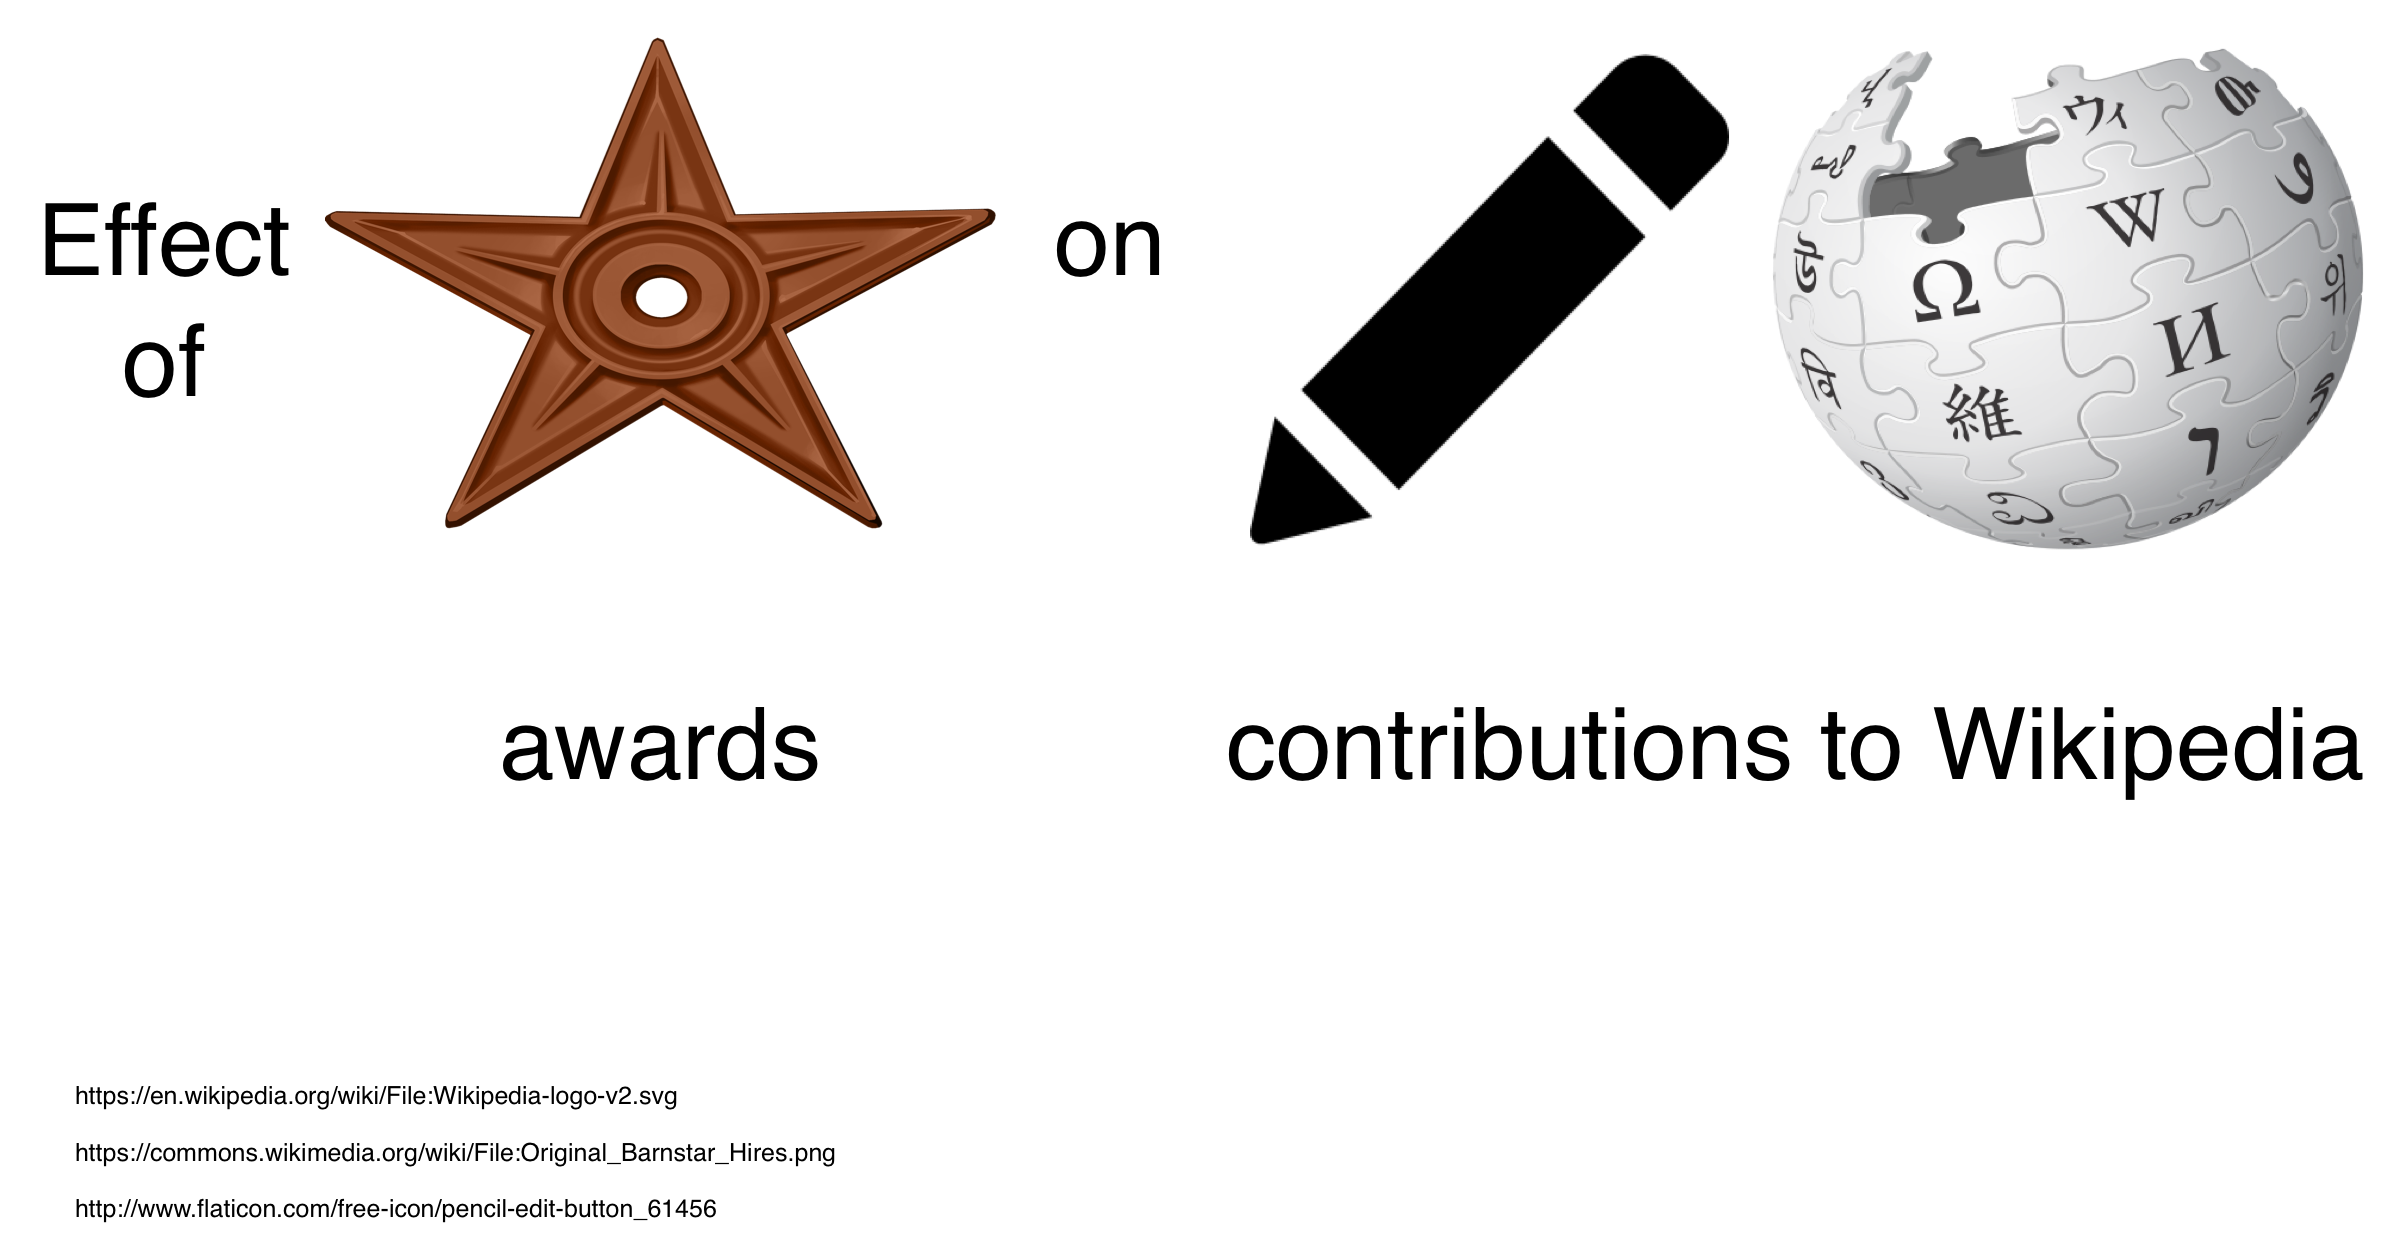
\includegraphics[width = \textwidth]{figures/restivo_experimental_2012_schematic}
\end{figure}

\end{frame}
%%%%%%%%%%%%%%%%%%%%%%%%%%%
\begin{frame}

What's the same?
\begin{itemize}
\item recruiting participants
\item randomization treatment
\item delivering treatment and control
\item measuring outcomes
\end{itemize}

\pause 
\vfill

What's different?
\begin{itemize}
\item Fully digital experiment leads to zero variable cost data.
\pause
\item Constraint on size is not cost, it is ethics.
\end{itemize}

\end{frame}
%%%%%%%%%%%%%%%%%%%%%%%%
\begin{frame}

Perturb and observe experiments vs randomized controlled experiments

\end{frame}
%%%%%%%%%%%%%%%%%%%%%%%%%%
\begin{frame}

``It's like you don't harass women, you don't steal, and you've got to have a control group. This is one of the things that you can lose your job for at Harrah's not running a control group.''
Gary Loveman, CEO Harrah's

\end{frame}
%%%%%%%%%%%%%%%%%%%%%%%%%%
\begin{frame}

\begin{itemize}
\item Sometimes we create a randomized controlled experiment by creating a treatment group 
\item Sometimes we create a randomized controlled experiment by creating a control group
\end{itemize}

\end{frame}
%%%%%%%%%%%%%%%%%%%%%%%%%%
\begin{frame}

\begin{center}
\only<1>{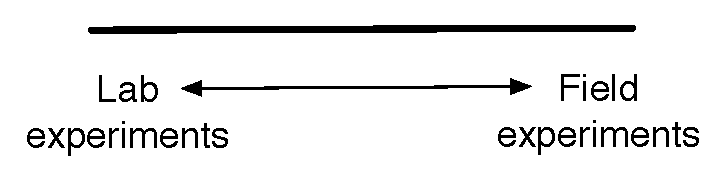
\includegraphics[width=0.7\textwidth]{figures/experiments_design_space_1d.pdf}}
\only<2>{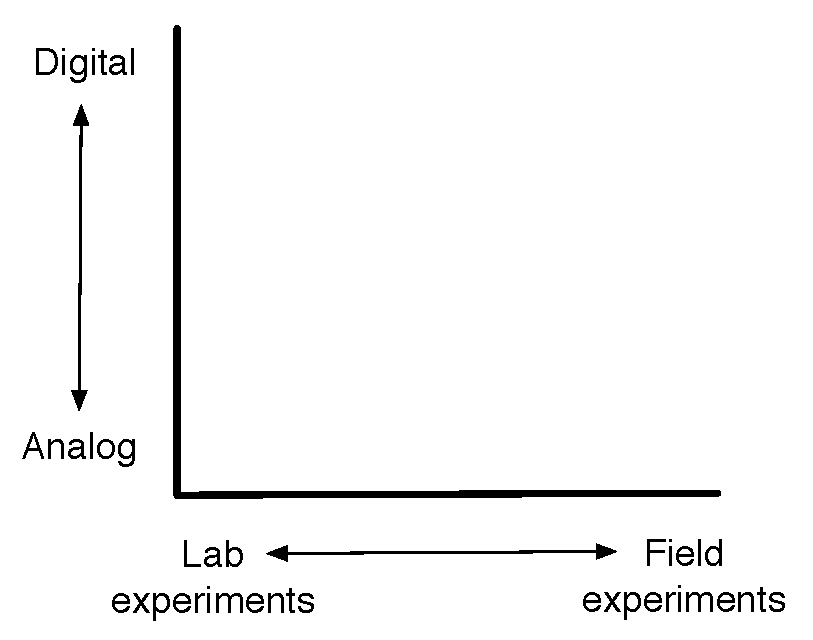
\includegraphics[width=0.7\textwidth]{figures/experiments_design_space_2d.pdf}}
\only<3>{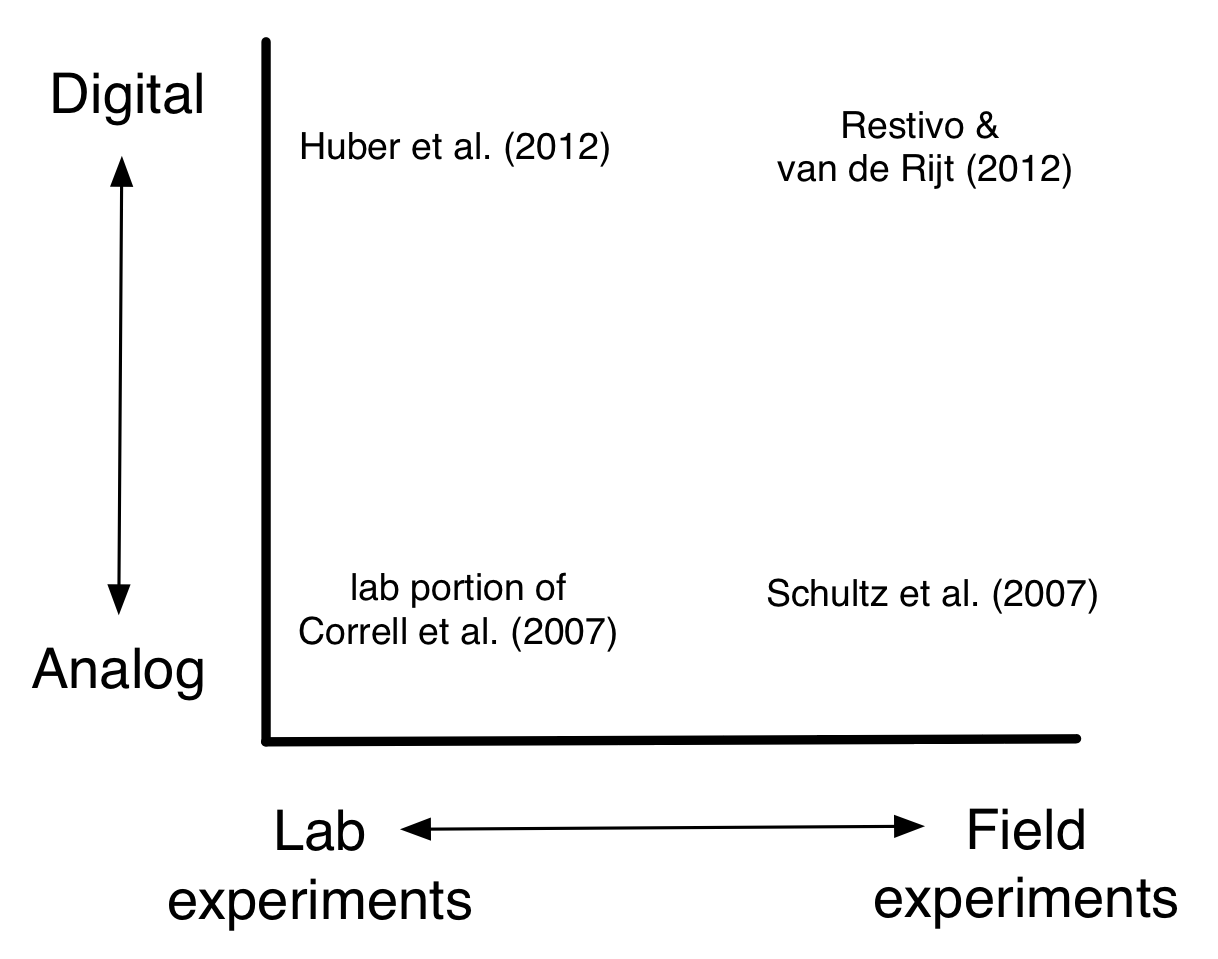
\includegraphics[width=0.7\textwidth]{figures/experiments_design_space}}
\end{center}

\end{frame}
%%%%%%%%%%%%%%%%%%%%%%%
\begin{frame}

\begin{center}
\LARGE Questions? 
\end{center}

\end{frame}
%%%%%%%%%%%%%%%%%%%%%%%%%%


\end{document}
